\section{BasketView}

Der Basket-View bildet alle Menüs und Produkte ab, die zuvor vom Nutzer zu dessen Warenkorb hinzugefügt
worden sind.

Hierfür wird für jede Ware ein \lstinline{Dismissible}-Widget verwendet. Dieses erlaubt dem Nutzer
ungewünschte Menüs und Produkte durch einen einfachen Swipe aus dem Warenkorb entfernt werden.
\cite{flutterDismissible}

\subsection{Dismissible-Widget für Ware}



\begin{code}[H]
    \centering
    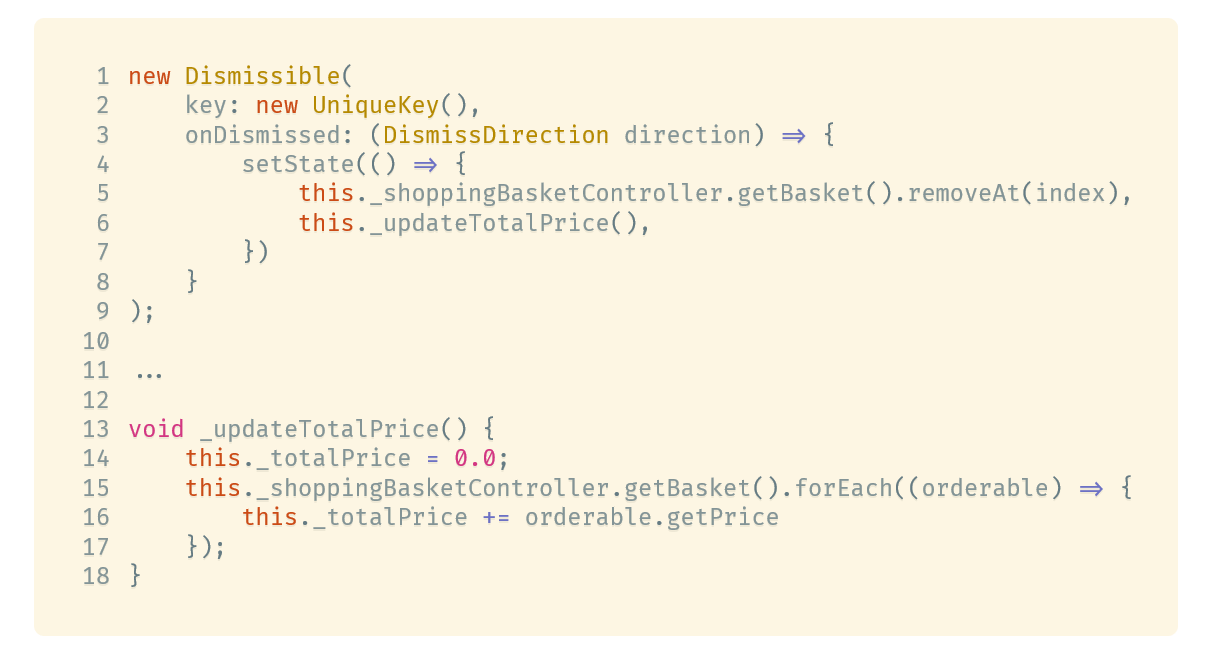
\includegraphics[width=1\textwidth]{images/Client/views/basketview/dismissible.png}
    \vspace{-20pt}
    \caption{Dismissible-Widget im Basket-View mit \lstinline{_updateTotalPrice}-Funktion zum Aktualisieren des Gesamtpreises}
\end{code}